\chapter{Technical details for hydrologic correction and synthesis}
\label{app:hydrology-technical}

This appendix preserves the detailed derivations, algorithms, and
secondary diagnostics supporting the corresponding research chapter.
The chapter retains the inferential target, central model, principal
evidence, interpretation, and limitations needed for a continuous read.

% migration-id: MIG-CH03-01
\section{Markov chain Monte Carlo algorithms}

The integrated algorithms use the same state-space notation as Subsection~\ref{env:subsec:fullmodel}. To keep the displays compact, they work with source-indexed observation vectors during the pre-cutoff observation window and with source-indexed forecast-product vectors during the forecast window. The role of the selector vector is therefore the same throughout: before the cutoff it is \(\mathbf{h}_{t,j}\), whereas after the cutoff it becomes the forecast-window selector \(\mathbf{e}_{T+k,j}\) for the active source \(j\). When the main text distinguishes individual forecast members through \(y_T^{j,i}(k)\), the integrated algorithms use the corresponding source-indexed forecast quantity \(y_{T+k}^{j}\) because the algorithms only need the active source channel at each lead time.

\begin{algorithmblock}{MCMC Algorithm}
\label{env:alg1}
\begingroup\scriptsize
\begin{algorithmic}

\STATE \textbf{Notation:}
\STATE  \(
A^j = A(\gamma^j;p_0), \quad B^j = B(\gamma^j;p_0), \quad C^j = C(\gamma^j;p_0), \text{ as defined in Subsection~\ref{env:subsec:exal}}
\)
\STATE Let \(\mathcal{J}_0=\{0\}\cup\mathcal{J}\), where \(j=0\) denotes the observation channel and \(j\in\mathcal{J}\) denotes an external source. During the pre-cutoff observation window, write \(y_t^0 \equiv y_t^o\) and \(y_t^j \equiv z_t^j\) for \(j\in\mathcal{J}\), with selector vector \(\mathbf{h}_{t,j}\). During the forecast window, write \(y_{T+k}^{j}\) for the active source-indexed forecast quantity from source \(j\) at lead \(k\), with selector \(\mathbf{e}_{T+k,j}\).
\STATE \textbf{Step 0: Set initial values} and sample size $N$.
\STATE Initialize $\{(v^j)^{(0)}_{1:T}, (s^j)^{(0)}_{1:T}, \boldsymbol{\eta}^{(0)}_{1:T}, (\sigma^j)^{(0)}, (\gamma^j)^{(0)}\}_{j\in\mathcal{J}_0}$
\FOR{$n = 1$ to $N$}
    \STATE \textbf{Step 1: Update $\boldsymbol{\eta}_t$}
    \STATE Use Algorithm~\ref{env:alg:Alg2}
    \FOR{$j \in \mathcal{J}_0$}
        \STATE \textbf{Step 2: Update $v^j_t$}
        \FOR{$t = 1$ to $T$}
            \STATE Sample $(v^j_t)^{(n)} \sim \mathcal{GIG}(a^j_t, b^j_t, c^j_t)$
            \STATE $a^j_t = \frac{1}{2}$
            \STATE $b^j_t = \frac{1}{(\sigma^j)^{(n-1)}}\left[ \frac{((A^j)^2)^{(n-1)}}{(B^j)^{(n-1)}}+2\right]$
            \STATE $c^j_t = \frac{1}{(\sigma^j)^{(n-1)} (B^j)^{(n-1)}}\left[y_t^j -\mathbf{h}_{t,j}' \boldsymbol{\eta}^{(n)}_t -(C^j)^{(n-1)} (\sigma^j)^{(n-1)} |(\gamma^j)^{(n-1)}| (s^j_t)^{(n-1)} \right]^2$
        \ENDFOR
        \IF{$j \in \mathcal{J}$}
        \FOR{$k = 1$ to $K_{(j)}$}
            \STATE Sample $(v^j_{T+k})^{(n)} \sim \mathcal{GIG}(a^j_{T+k}, b^j_{T+k}, c^j_{T+k})$
            \STATE $a^j_{T+k} = \frac{1}{2}$
            \STATE $b^j_{T+k} = \frac{1}{(\sigma^j)^{(n-1)}}\left[ \frac{((A^j)^2)^{(n-1)}}{(B^j)^{(n-1)}}+2\right]$
            \STATE $r^j_{T+k}=y_{T+k}^j-\mathbf{e}_{T+k,j}'\boldsymbol{\eta}^{(n)}_{T+k}
            -(C^j)^{(n-1)}(\sigma^j)^{(n-1)}|(\gamma^j)^{(n-1)}|(s^j_{T+k})^{(n-1)}$
            \STATE $c^j_{T+k}=\{r^j_{T+k}\}^2/
            \{(\sigma^j)^{(n-1)}(B^j)^{(n-1)}\}$
        \ENDFOR
        \ENDIF

        \STATE \textbf{Step 3: Update $s^j_t$}
        \FOR{$t = 1$ to $T$}
            \STATE Sample $(s^j)^{(n)}_t \sim \mathcal{N}^+(m^j_t, \lambda^j_t)$
            \STATE $\lambda^j_t =  \left[\frac{\big((C^j)^{(n-1)}(\gamma^j)^{(n-1)} \big)^2(\sigma^j)^{(n-1)}}{(B^j)^{(n-1)}(v^j_t)^{(n)}}+1\right]$
            \STATE $m^j_t =  \lambda^j_t \left[\frac{(C^j)^{(n-1)}|(\gamma^j)^{(n-1)}|(y_t^j -\mathbf{h}_{t,j}' \boldsymbol{\eta}^{(n)}_t - (A^j)^{(n-1)} (v^j_t)^{(n)})}{(B^j)^{(n-1)}(v^j_t)^{(n)}}\right]$
        \ENDFOR

        \STATE \textbf{Step 4: Update $\sigma^j$}
        \STATE Sample $(\sigma^j)^{(n)} \sim \mathcal{GIG}(a^j_t, b^j_t, c^j_t)$
        \STATE $a^j_t = -(1.5T + a_{\sigma^j})$
        \STATE $b^j_t = \sum_{t=1}^T \frac{1}{(B^j)^{(n-1)} (v^j_t)^{(n)}} \left((C^j)^{(n-1)} |(\gamma^j)^{(n-1)}| (s^j_t)^{(n)} \right)^2$
        \STATE $c^j_t = \sum_{t=1}^T \frac{1}{(B^j)^{(n-1)} (v^j_t)^{(n)}}\big(y_t^j -\mathbf{h}_{t,j}' \boldsymbol{\eta}^{(n)}_t - (A^j)^{(n-1)} (v^j_t)^{(n)}\big)^2 + 2 \sum_{t=1}^T  (v^j_t)^{(n)} + 2 b_{\sigma^j}$

        \STATE \textbf{Step 5: Update $\gamma^j$}
        \STATE Implement Metropolis-Hastings (MH)
    \ENDFOR
\ENDFOR

\end{algorithmic}
\endgroup
\end{algorithmblock}

\begin{algorithmblock}{MCMC - Forward Filtering Backward Sampling (FFBS)}
\label{env:alg:Alg2}
\begingroup\scriptsize
\begin{algorithmic}

\STATE \textbf{Notation:}
\STATE  During the pre-cutoff observation window, \(\mathbf{H}_t = [\mathbf{h}_{t,0}, \mathbf{h}_{t,1}, \ldots, \mathbf{h}_{t,J}]\), \(\mathbf{Y}_t = [y_t^o, z_t^1, \ldots, z_t^J]'\), and \(\mathbf{D}_t, \boldsymbol{\Lambda}_t\) are as defined in Subsection~\ref{env:subsec:fullmodel}.
\STATE  Equivalently, \(y_t^0 \equiv y_t^o\) and \(y_t^j \equiv z_t^j\) for \(j\in\mathcal{J}\), so the filtering recursion can be written in source-indexed form.
\STATE $\mathbf{M}_t= \mathbf{C} \odot  \mathbf{\sigma} \odot | \mathbf{\gamma} | \odot \mathbf{s}_t + \mathbf{A} \odot \mathbf{v}_t$, \quad $\mathbf{O}_t= \sqrt{\mathbf{B} \odot \mathbf{v}_t} \odot Diag
(\mathbf{\sigma}) \sqrt{\mathbf{B} \odot \mathbf{v}_t} \odot \mathbf{\sigma}$
\STATE  \(
\mathbf{A} = \big[ A(\gamma^j;p_0)   \big], \quad \mathbf{B} = \big[  B(\gamma^j;p_0)  \big], \quad \mathbf{C} = \big[ C(\gamma^j;p_0)   \big] \), \text{ as defined in Subsection~\ref{env:subsec:exal}}
\STATE \( \mathbf{v}_t = \big[  v^j_t   \big], \quad  \mathbf{s}_t = \big[
s^j_t  \big] , \quad \mathbf{\sigma} = \big[ \sigma^j  \big]
\)
\STATE \(\odot\) denotes the Hadamard product.
\STATE \textbf{Step 1: Forward Filtering}
\FOR{$t = 1$ to $T$}
    \STATE Compute Prior moments:
    \STATE $\mathbf{a}_t = \mathbf{D}_t \mathbf{m}_{t-1}$
    \STATE $\mathbf{R}_t = \mathbf{D}_t \mathbf{C}_{t-1} \mathbf{D}_t' +  \boldsymbol{\Lambda}_t$

    \STATE One-step-ahead forecast:
    \STATE $\mathbf{f}_t = \mathbf{H}_t' \mathbf{a}_t + \mathbf{M}_t$
    \STATE $\mathbf{Q}_t = \mathbf{H}_t' \mathbf{R}_t \mathbf{H}_t + \mathbf{O}_t$

    \STATE Compute Posterior moments:
    \STATE $\mathbf{m}_t = \mathbf{a}_t + \mathbf{R}_t \mathbf{H}_t \mathbf{Q}_t^{-1}(\mathbf{Y}_t - \mathbf{f}_t)$
    \STATE $\mathbf{C}_t = \mathbf{R}_t - \mathbf{R}_t \mathbf{H}_t \mathbf{Q}_t^{-1} \mathbf{H}_t' \mathbf{R}_t$
\ENDFOR

\STATE \textbf{Step 2: Backward Sampling}
\FOR{$t = T$ down to $0$}
    \IF{$t = T$}
        \STATE Sample $\boldsymbol{\eta}_T | D_T \sim \mathcal{N}(\mathbf{m}_T, \mathbf{C}_T)$
    \ELSE
        \STATE Compute Retrospective moments:
        \STATE $\mathbf{m}_t^s = \mathbf{m}_t + \mathbf{C}_t \mathbf{D}_{t+1}' \mathbf{R}_{t+1}^{-1} (\boldsymbol{\eta}_{t+1} - \mathbf{a}_{t+1})$
        \STATE $\mathbf{C}_t^s = \mathbf{C}_t - \mathbf{C}_t \mathbf{D}_{t+1}' \mathbf{R}_{t+1}^{-1} \mathbf{D}_{t+1} \mathbf{C}_t$

        \STATE Sample $\boldsymbol{\eta}_t | D_T \sim \mathcal{N}(\mathbf{m}_t^s, \mathbf{C}_t^s)$
    \ENDIF
\ENDFOR

\end{algorithmic}
\endgroup
\end{algorithmblock}

 \clearpage

\section{Variational Bayes algorithms}

\begin{algorithmblock}{Variational Bayes (VB) Algorithm}
\label{env:alg:Alg3}
\begingroup\scriptsize
\begin{algorithmic}

\STATE \textbf{Notation:}
\STATE  $\left\langle g(\xi) \right\rangle = \mathbb{E}_\xi\left[ g(\xi) \right]$
\STATE  \(
A^j = A(\gamma^j;p_0), \quad B^j = B(\gamma^j;p_0), \quad C^j = C(\gamma^j;p_0), \text{ as defined in Subsection~\ref{env:subsec:exal}}
\)
\STATE  Let \(\mathcal{J}_0=\{0\}\cup\mathcal{J}\). During the pre-cutoff observation window, let \(y_t^0 \equiv y_t^o\) and \(y_t^j \equiv z_t^j\) for \(j\in\mathcal{J}\), with selector \(\mathbf{h}_{t,j}\). This is the same source-indexed notation used in Algorithm~\ref{env:alg1}.
\STATE \textbf{Step 0: Set initial values}
\STATE Choose \(k_{\max}\), minimum update counts, and convergence tolerances; set \(k=0\)

\WHILE{\(k < k_{\max}\) and convergence criteria are not met}
    \STATE \(k \leftarrow k+1\)
    \STATE \textbf{Step 1: Update $r(\boldsymbol{\eta}_t)=\mathcal{N}(m^{(k)}_t,C^{(k)}_t)$}
    \STATE Use Algorithm~\ref{env:alg:Alg4}

    \FOR{$j \in \mathcal{J}_0$}
        \STATE \textbf{Step 2: Update $r(v^j_t)=\mathcal{GIG}(a_t^{j,(k)},b_t^{j,(k)},c_t^{j,(k)})$}
        \FOR{$t = 1$ to $T$}
            \STATE $a_t^{j,(k)} = \frac{1}{2}$
            \STATE $b_t^{j,(k)} = \left\langle \frac{A^2}{\sigma^j B^j} \right\rangle^{(k-1)} + 2 \left\langle \frac{1}{\sigma^j} \right\rangle^{(k-1)}$
            \STATE $c_t^{j,(k)} = \left\langle \frac{1}{\sigma^j B^j} \right\rangle^{(k-1)} \Big[ (y_t^j)^2 - 2y_t^j \left\langle  \mathbf{h}_{t,j}' \boldsymbol{\eta}_t \right\rangle^{(k)} + \left\langle (  \mathbf{h}_{t,j}' \boldsymbol{\eta}_t )^2 \right\rangle^{(k)} \Big]$
            \STATE $\quad \quad -2 \left\langle s^j_t \right\rangle^{(k-1)} \left\langle \frac{C^j|\gamma^j|}{B^j} \right\rangle^{(k-1)} \Big[ y_t^j - \left\langle  \mathbf{h}_{t,j}' \boldsymbol{\eta}_t \right\rangle^{(k)} \Big]$
            \STATE $\quad \quad + \left\langle (s^j_t)^2 \right\rangle^{(k-1)} \left\langle \frac{(C^j)^2\sigma^j|\gamma^j|^2}{B^j} \right\rangle^{(k-1)}$
        \ENDFOR

        \STATE \textbf{Step 3: Update $r(s^j_t)=\mathcal{N}^+(\eta^{j,(k)},\lambda^{j,(k)})$}
        \FOR{$t = 1$ to $T$}
            \STATE $\lambda^{j,(k)} = \Big[ 1+\left\langle \frac{(C^j)^2 \sigma^j |(\gamma^j)|^2}{B^j} \right\rangle^{(k-1)} \left\langle \frac{1}{v^j_t} \right\rangle^{(k)} \Big]^{-1}$
            \STATE $\eta^{j,(k)} = \lambda^{j,(k)}  \Big[ \left\langle \frac{C^j |\gamma^j|}{B^j} \right\rangle^{(k-1)} \left\langle \frac{1}{v^j_t} \right\rangle^{(k)} \Big( y_t^j - \left\langle  \mathbf{h}_{t,j}' \boldsymbol{\eta}_t \right\rangle^{(k)} \Big) - \left\langle \frac{C^j |\gamma^j| A^j}{B^j} \right\rangle^{(k-1)} \Big]$
        \ENDFOR

        \STATE \textbf{Step 4: Update $r(\gamma^j, \sigma^j )$}
        \STATE Approximate via VB-LD, as described in Subsection~\ref{env:subsec:postinf}
    \ENDFOR
    \STATE \textbf{Step 5: Check convergence}
    \STATE Compute \(\mathcal{L}^{(k)}\), \(\Delta_{\mathcal{L}}^{(k)}=|\mathcal{L}^{(k)}-\mathcal{L}^{(k-1)}|\), and the relative ELBO change
    \STATE Declare convergence after required update iterations when ELBO,
    \STATE \hspace{\algorithmicindent} state, scale, and skewness changes are below their tolerances
\ENDWHILE

\end{algorithmic}
\endgroup
\end{algorithmblock}

\begin{algorithmblock}{VB-Filtering and VB-Smoothing}
\label{env:alg:Alg4}
\begingroup\scriptsize
\begin{algorithmic}

\STATE \textbf{Notation:}
\STATE $\left\langle g(\xi) \right\rangle = \mathbb{E}_\xi\left[ g(\xi) \right]$
\STATE  During the pre-cutoff observation window, \(\mathbf{H}_t = [\mathbf{h}_{t,0}, \mathbf{h}_{t,1}, \ldots, \mathbf{h}_{t,J}]\), \(\mathbf{Y}_t = [y_t^o, z_t^1, \ldots, z_t^J]'\), and \(\mathbf{D}_t, \boldsymbol{\Lambda}_t\) are as defined in Subsection~\ref{env:subsec:fullmodel}.
\STATE  Equivalently, let \(y_t^0 \equiv y_t^o\) and \(y_t^j \equiv z_t^j\) for \(j\in\mathcal{J}\). This algorithm is the variational analogue of Algorithm~\ref{env:alg:Alg2}.
\STATE $\mathbf{M}_t= \mathbf{C} \odot  \mathbf{\sigma} \odot | \mathbf{\gamma} | \odot \mathbf{s}_t + \mathbf{A} \odot \mathbf{v}_t$, \quad $\mathbf{O}_t= \sqrt{\mathbf{B} \odot \mathbf{v}_t} \odot Diag
(\mathbf{\sigma}) \sqrt{\mathbf{B} \odot \mathbf{v}_t} \odot \mathbf{\sigma}$
\STATE \(\mathbf{A}=\big[\left\langle A(\gamma^j;p_0)\right\rangle\big]\),
\STATE \(\mathbf{B}=\big[\left\langle B(\gamma^j;p_0)\right\rangle\big]\), and
\STATE \(\mathbf{C}=\big[\left\langle C(\gamma^j;p_0)\right\rangle\big]\), as defined in Subsection~\ref{env:subsec:exal}.
\STATE \( \mathbf{v}_t = \big[ \left\langle v^j_t  \right\rangle \big], \quad  \mathbf{s}_t = \big[ \left\langle
s^j_t  \right\rangle \big] , \quad \mathbf{\sigma} = \big[ \left\langle \sigma^j  \right\rangle \big]
\)
\STATE \(\odot\) denotes the Hadamard product.
\STATE \textbf{Step 1: Forward Filtering}
\FOR{$t = 1$ to $T$}
    \STATE Compute Prior moments:
    \STATE $\mathbf{a}_t = \mathbf{D}_t \mathbf{m}_{t-1}$
    \STATE $\mathbf{R}_t = \mathbf{D}_t \mathbf{C}_{t-1} \mathbf{D}_t' +  \boldsymbol{\Lambda}_t$

    \STATE One-step-ahead forecast:
    \STATE $\mathbf{f}_t = \mathbf{H}_t'\mathbf{a}_t + \mathbf{M}_t$
    \STATE $\mathbf{Q}_t = \mathbf{H}_t'\mathbf{R}_t\mathbf{H}_t + \mathbf{O}_t$

    \STATE Compute Posterior moments:
    \STATE $\mathbf{m}_t = \mathbf{a}_t + \mathbf{R}_t \mathbf{H}_t \mathbf{Q}_t^{-1}(\mathbf{Y}_t - \mathbf{f}_t)$
    \STATE $\mathbf{C}_t = \mathbf{R}_t - \mathbf{R}_t \mathbf{H}_t \mathbf{Q}_t^{-1} \mathbf{H}_t' \mathbf{R}_t$
\ENDFOR

\STATE \textbf{Step 2: Backward Smoothing}
\FOR{$t = T$ down to $1$}
    \IF{$t = T$}
        \STATE Set $r^{(k+1)}(\boldsymbol{\eta}_T) := \mathcal{N}(\mathbf{m}_T^s, \mathbf{C}_T^s)$
        \STATE $\mathbf{m}_T^s = \mathbf{m}_T$
        \STATE $\mathbf{C}_T^s = \mathbf{C}_T$
    \ELSE
        \STATE Compute Smoothing moments:
        \STATE $r^{(k+1)}(\boldsymbol{\eta}_t) := \mathcal{N}(\mathbf{m}_t^s, \mathbf{C}_t^s)$
        \STATE $B_t = \mathbf{C}_t \mathbf{D}_{t+1}' \mathbf{R}_{t+1}^{-1}$
        \STATE $\mathbf{m}_t^s = \mathbf{m}_t + \mathbf{B}_t (\mathbf{m}_{t+1}^s - \mathbf{a}_{t+1})$
        \STATE $\mathbf{C}_t^s = \mathbf{C}_t + \mathbf{B}_t (\mathbf{C}_{t+1}^s - \mathbf{R}_{t+1}) \mathbf{B}_t'$
    \ENDIF
\ENDFOR


\end{algorithmic}
\endgroup
\end{algorithmblock}

% migration-id: MIG-CH03-02
\section{Source-specific exAL parameter summaries}
\label{env:app:sourceparams}

At the representative December 25, 2022 cutoff, the posterior medians of the
source-specific exAL skewness parameter decrease across the fitted quantile
grid. For USGS they range from 0.845 at the 0.05 level to -2.138 at the 0.95
level; the corresponding GloFAS values range from 0.975 to -0.728, and the NWS
values from 0.481 to -1.492. The posterior median scale parameters are smaller
near the two tails than near the central quantiles. Across the seven fitted
levels, the USGS scale ranges from 0.029 to 0.081, the GloFAS scale from 0.021
to 0.053, and the NWS scale from 0.028 to 0.108. These are parameters of the
source-specific exAL likelihoods, not weights assigned to the sources in the
predictive synthesis. The full posterior intervals remain recorded in the
fixed source materials but do not require separate dissertation tables.

\section{Cutoff-specific predictive synthesis panels}
\label{env:app:cutoffsynthpanels}

The main text shows the December 25, 2022 synthesis as a representative selected-model illustration. For completeness, this section reports the corresponding multivariate synthesis panels for the other rolling-origin cutoffs. Each panel uses the same exAL-M-T1 synthesis specification as Figure~\ref{env:fig:synth1} and includes the retrospective and forecast-product references used at that cutoff.

\begin{figure}[p]
\centering
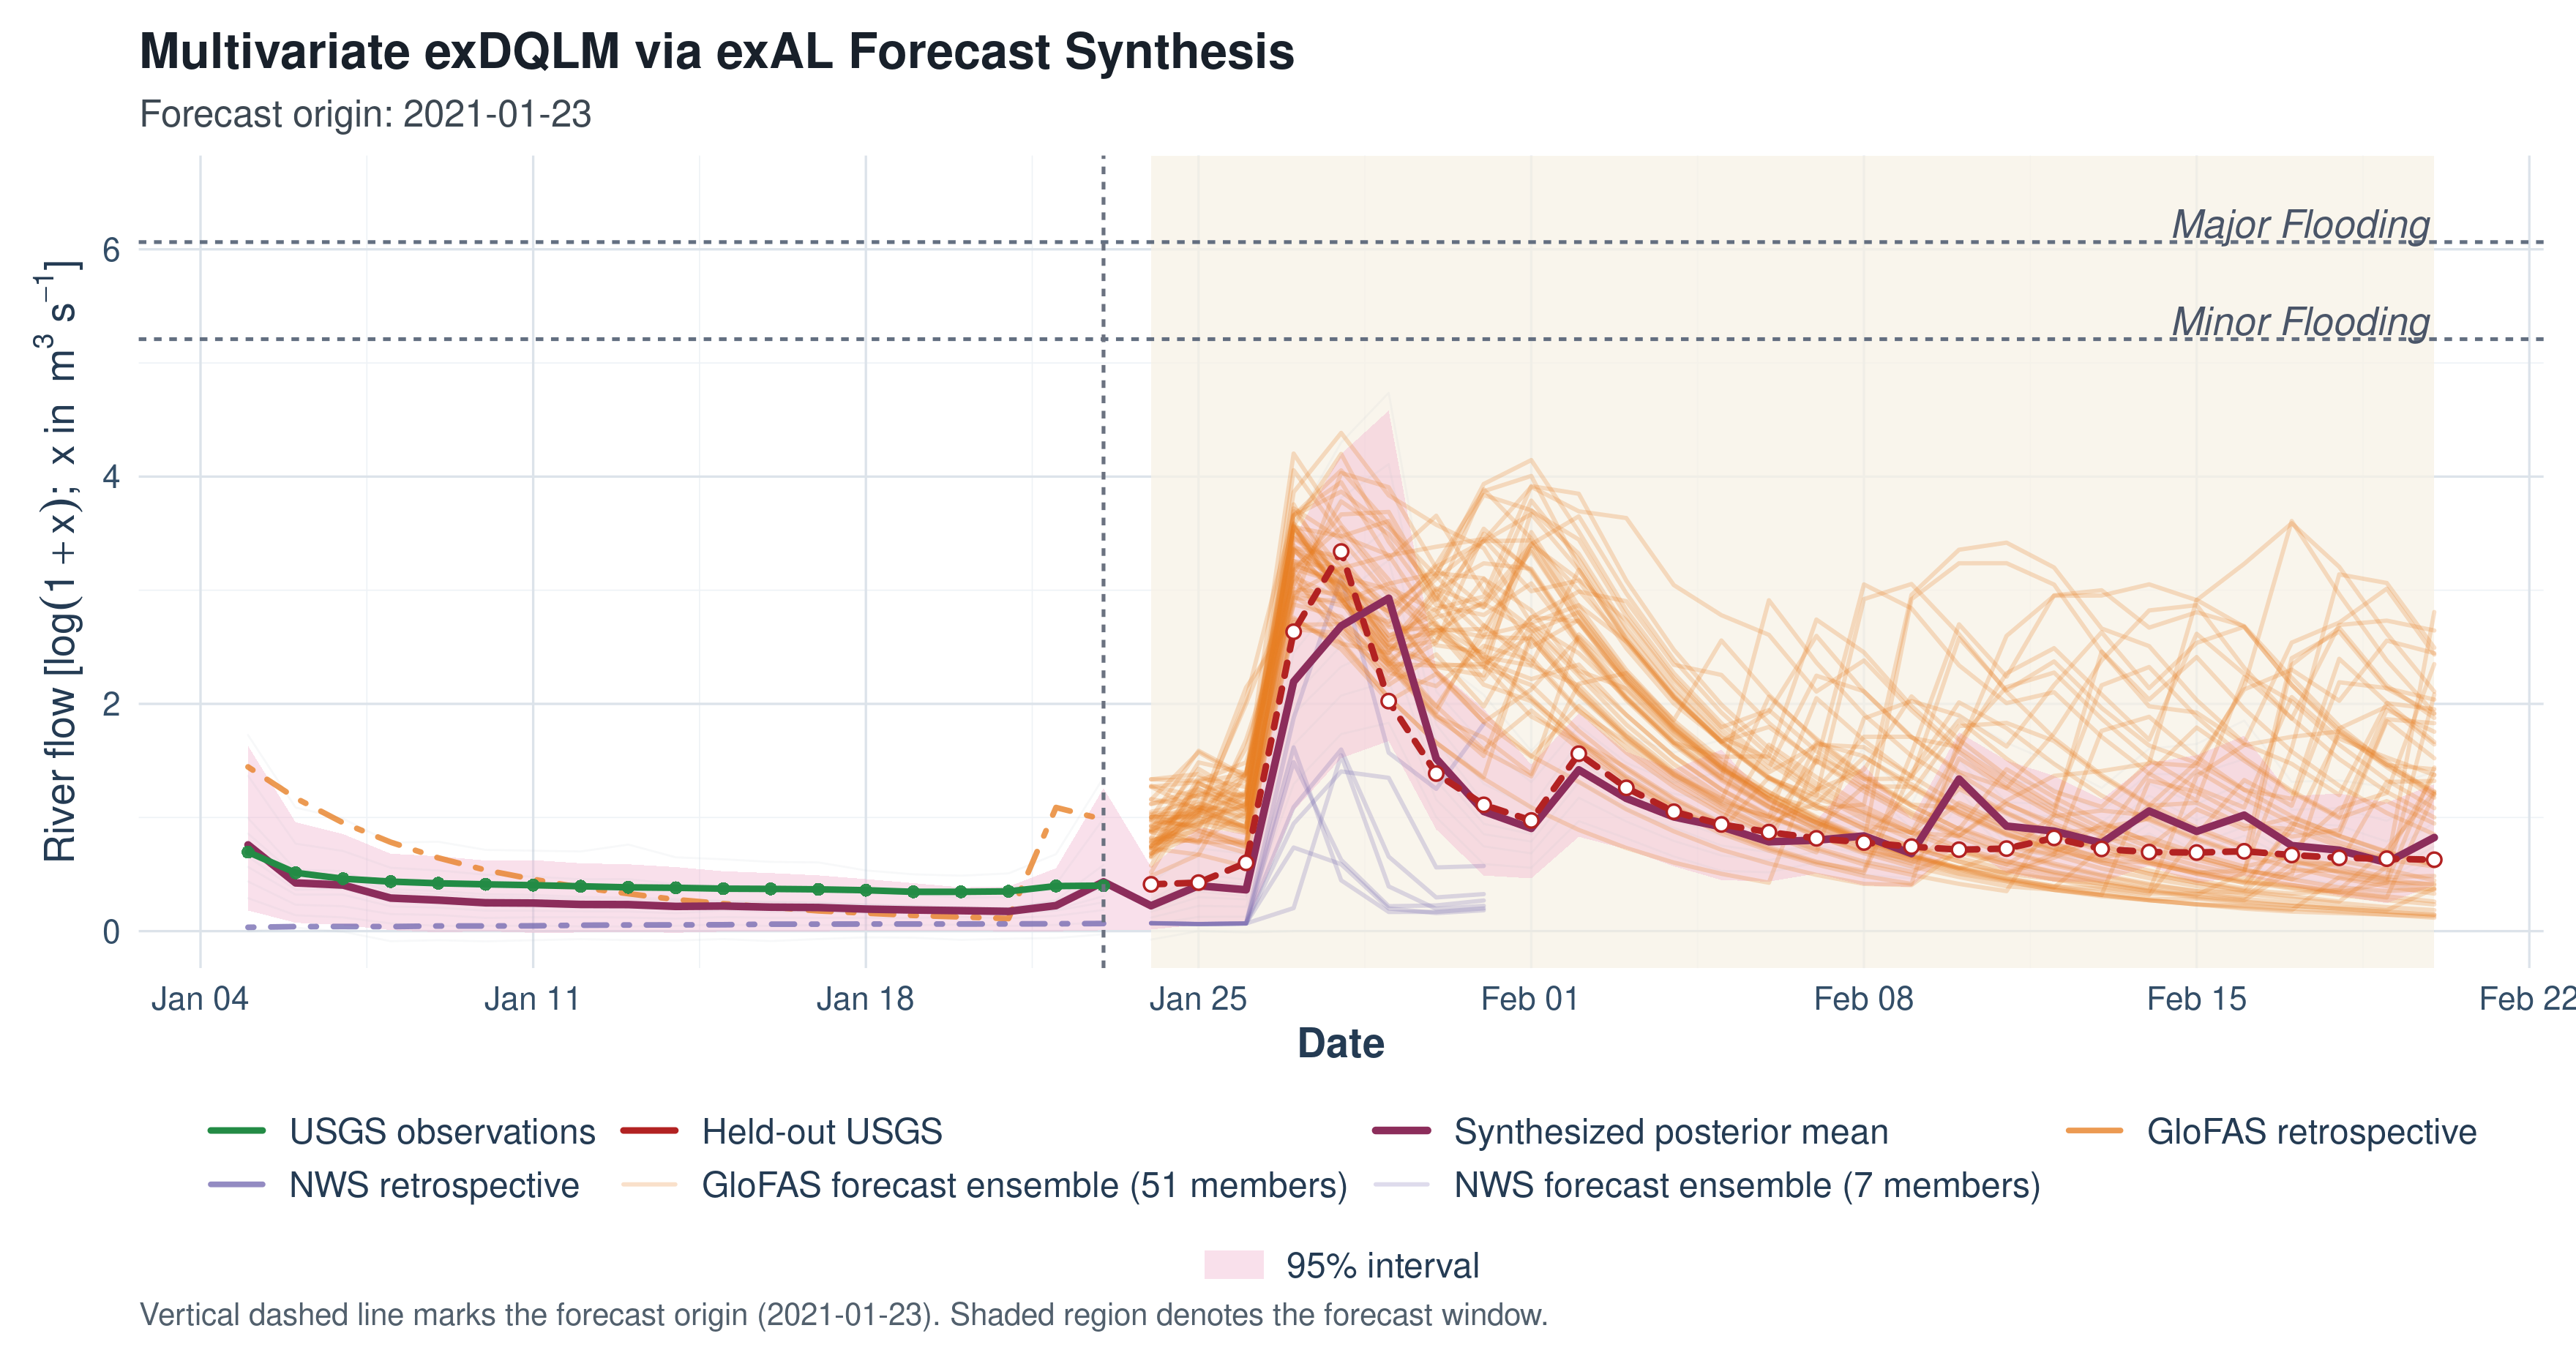
\includegraphics[width=0.76\textwidth]{figures/ch03-environ/cutoff_2021_01_23_multivariate_synthesis_with_reference_ensembles.png}

\medskip
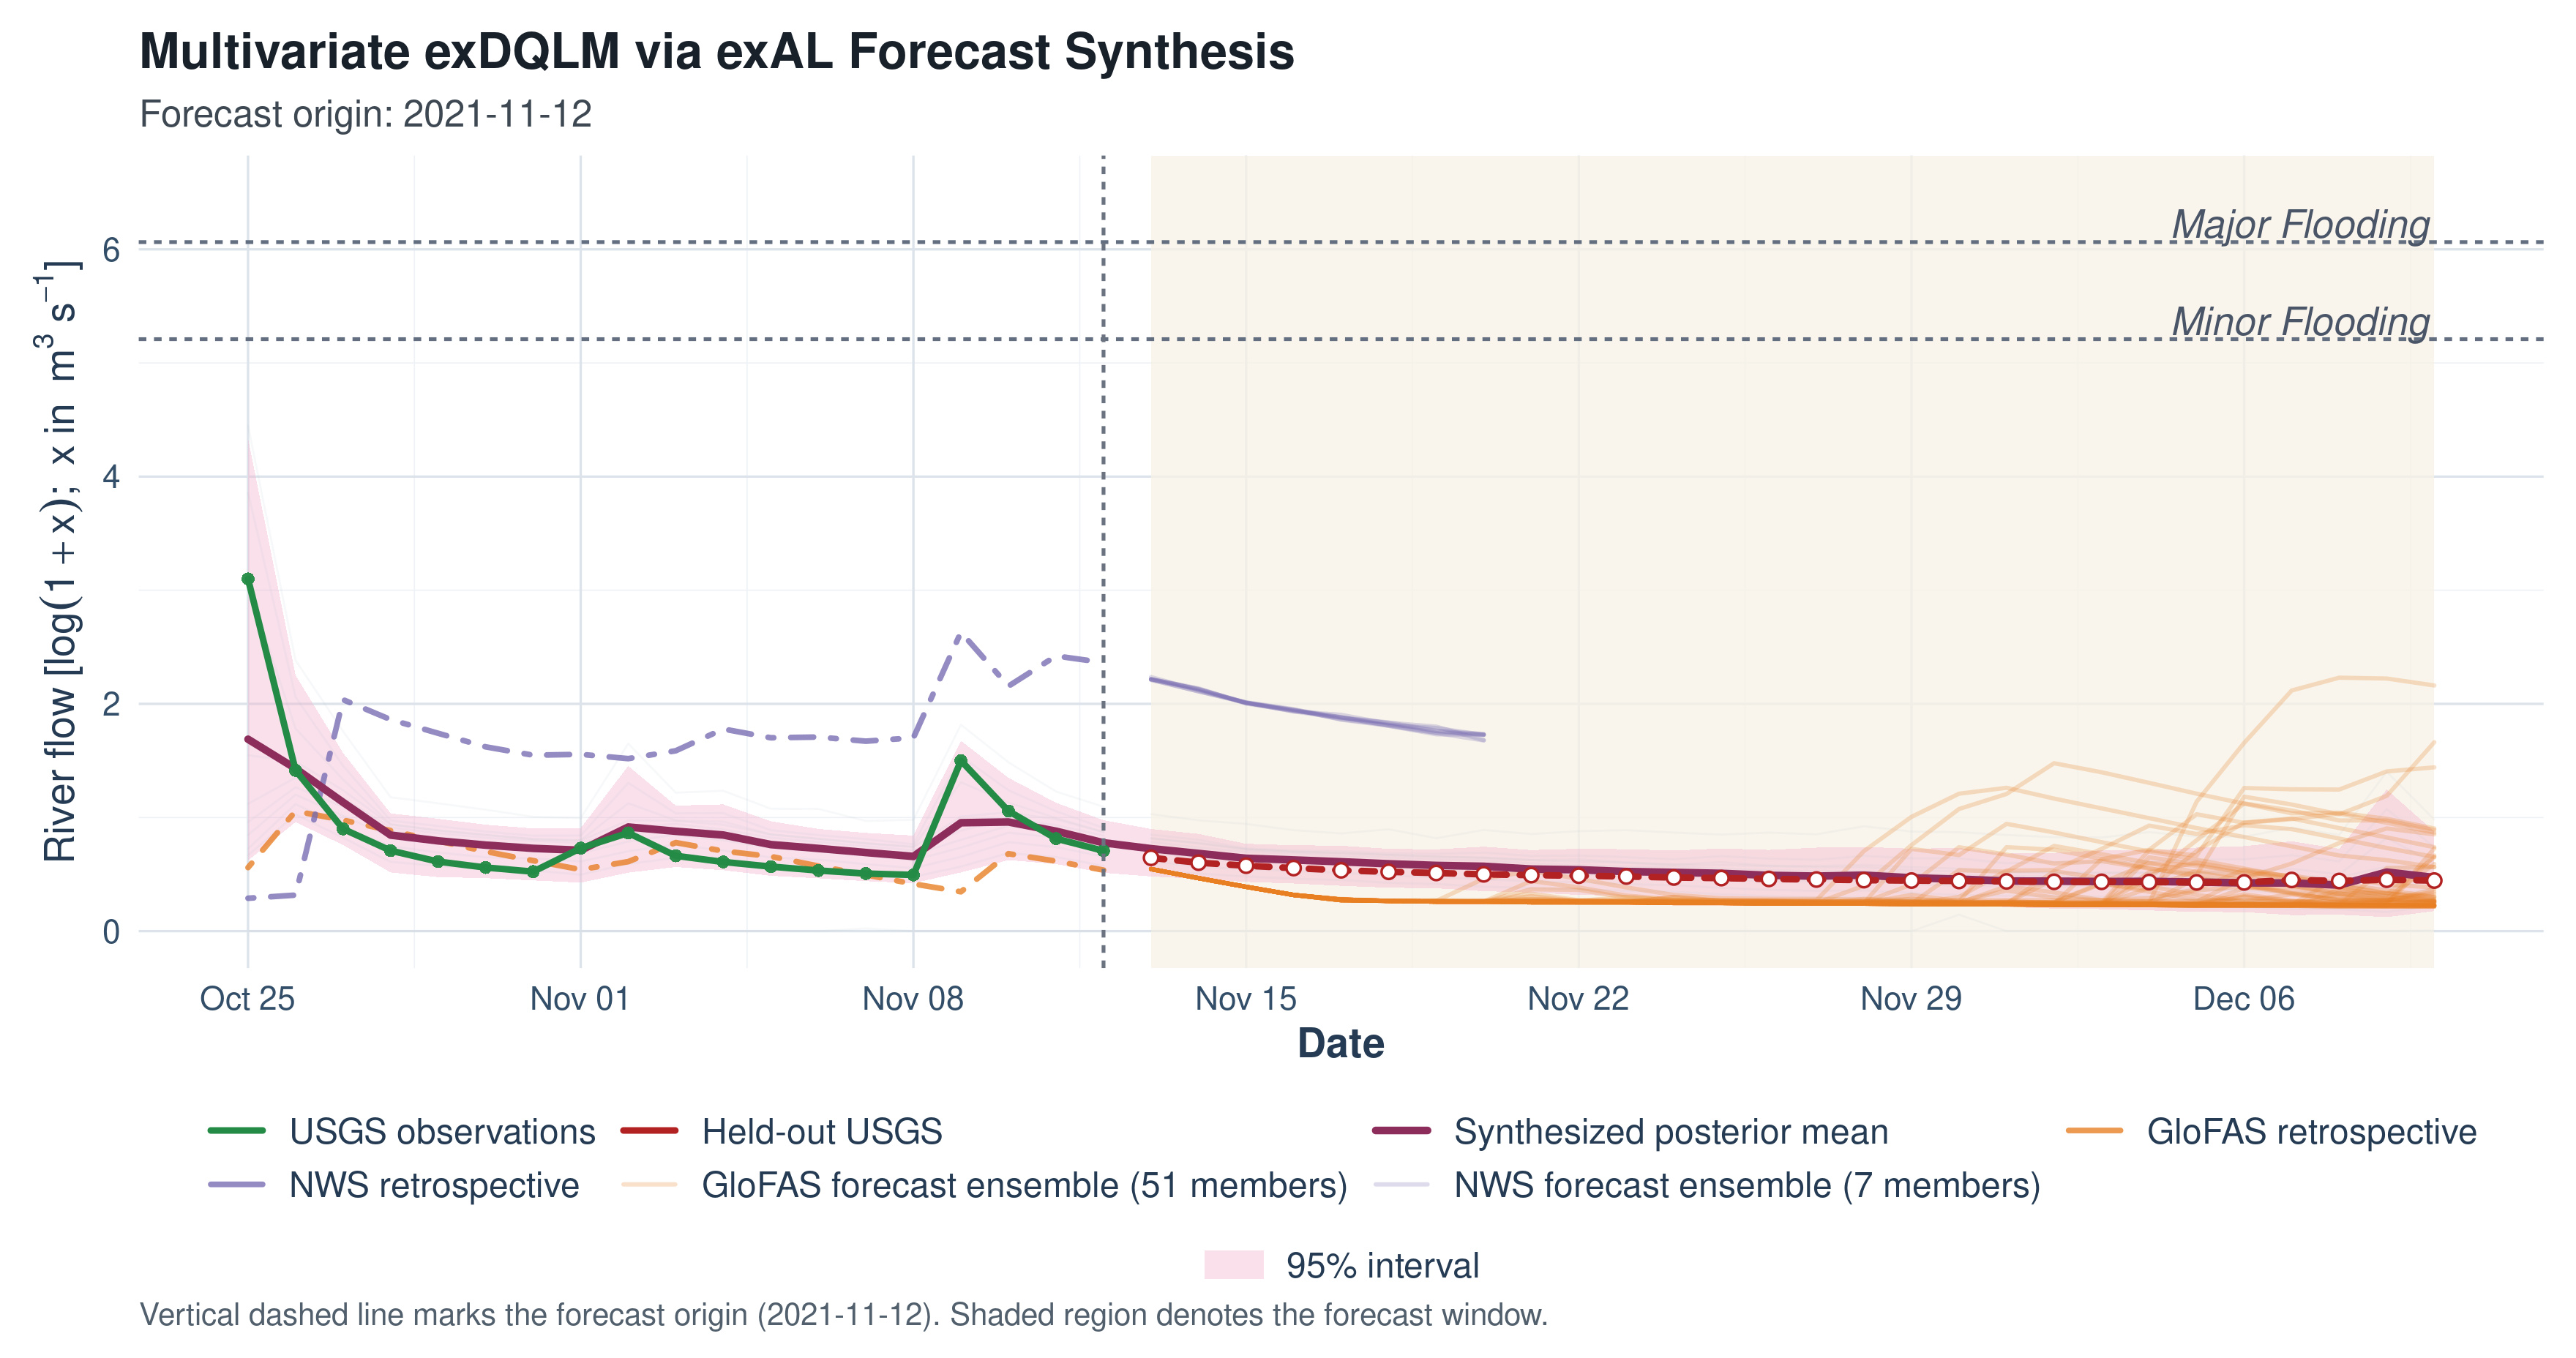
\includegraphics[width=0.76\textwidth]{figures/ch03-environ/cutoff_2021_11_12_multivariate_synthesis_with_reference_ensembles.png}
\caption[Predictive synthesis at the January and November 2021 cutoffs]{
Predictive synthesis under exAL-M-T1 at the January 23 (upper) and November 12,
2021 (lower) cutoffs. Green denotes pre-origin USGS measurements, red denotes
held-out USGS verification, the pink region is the central 95\% posterior
predictive band, and thin lines are the seven displayed synthesized quantiles.
Raw retrospective and forecast products provide cutoff-specific reference
overlays.
}
\label{env:fig:synthsupport_20210123}
\end{figure}

\begin{figure}[p]
\centering
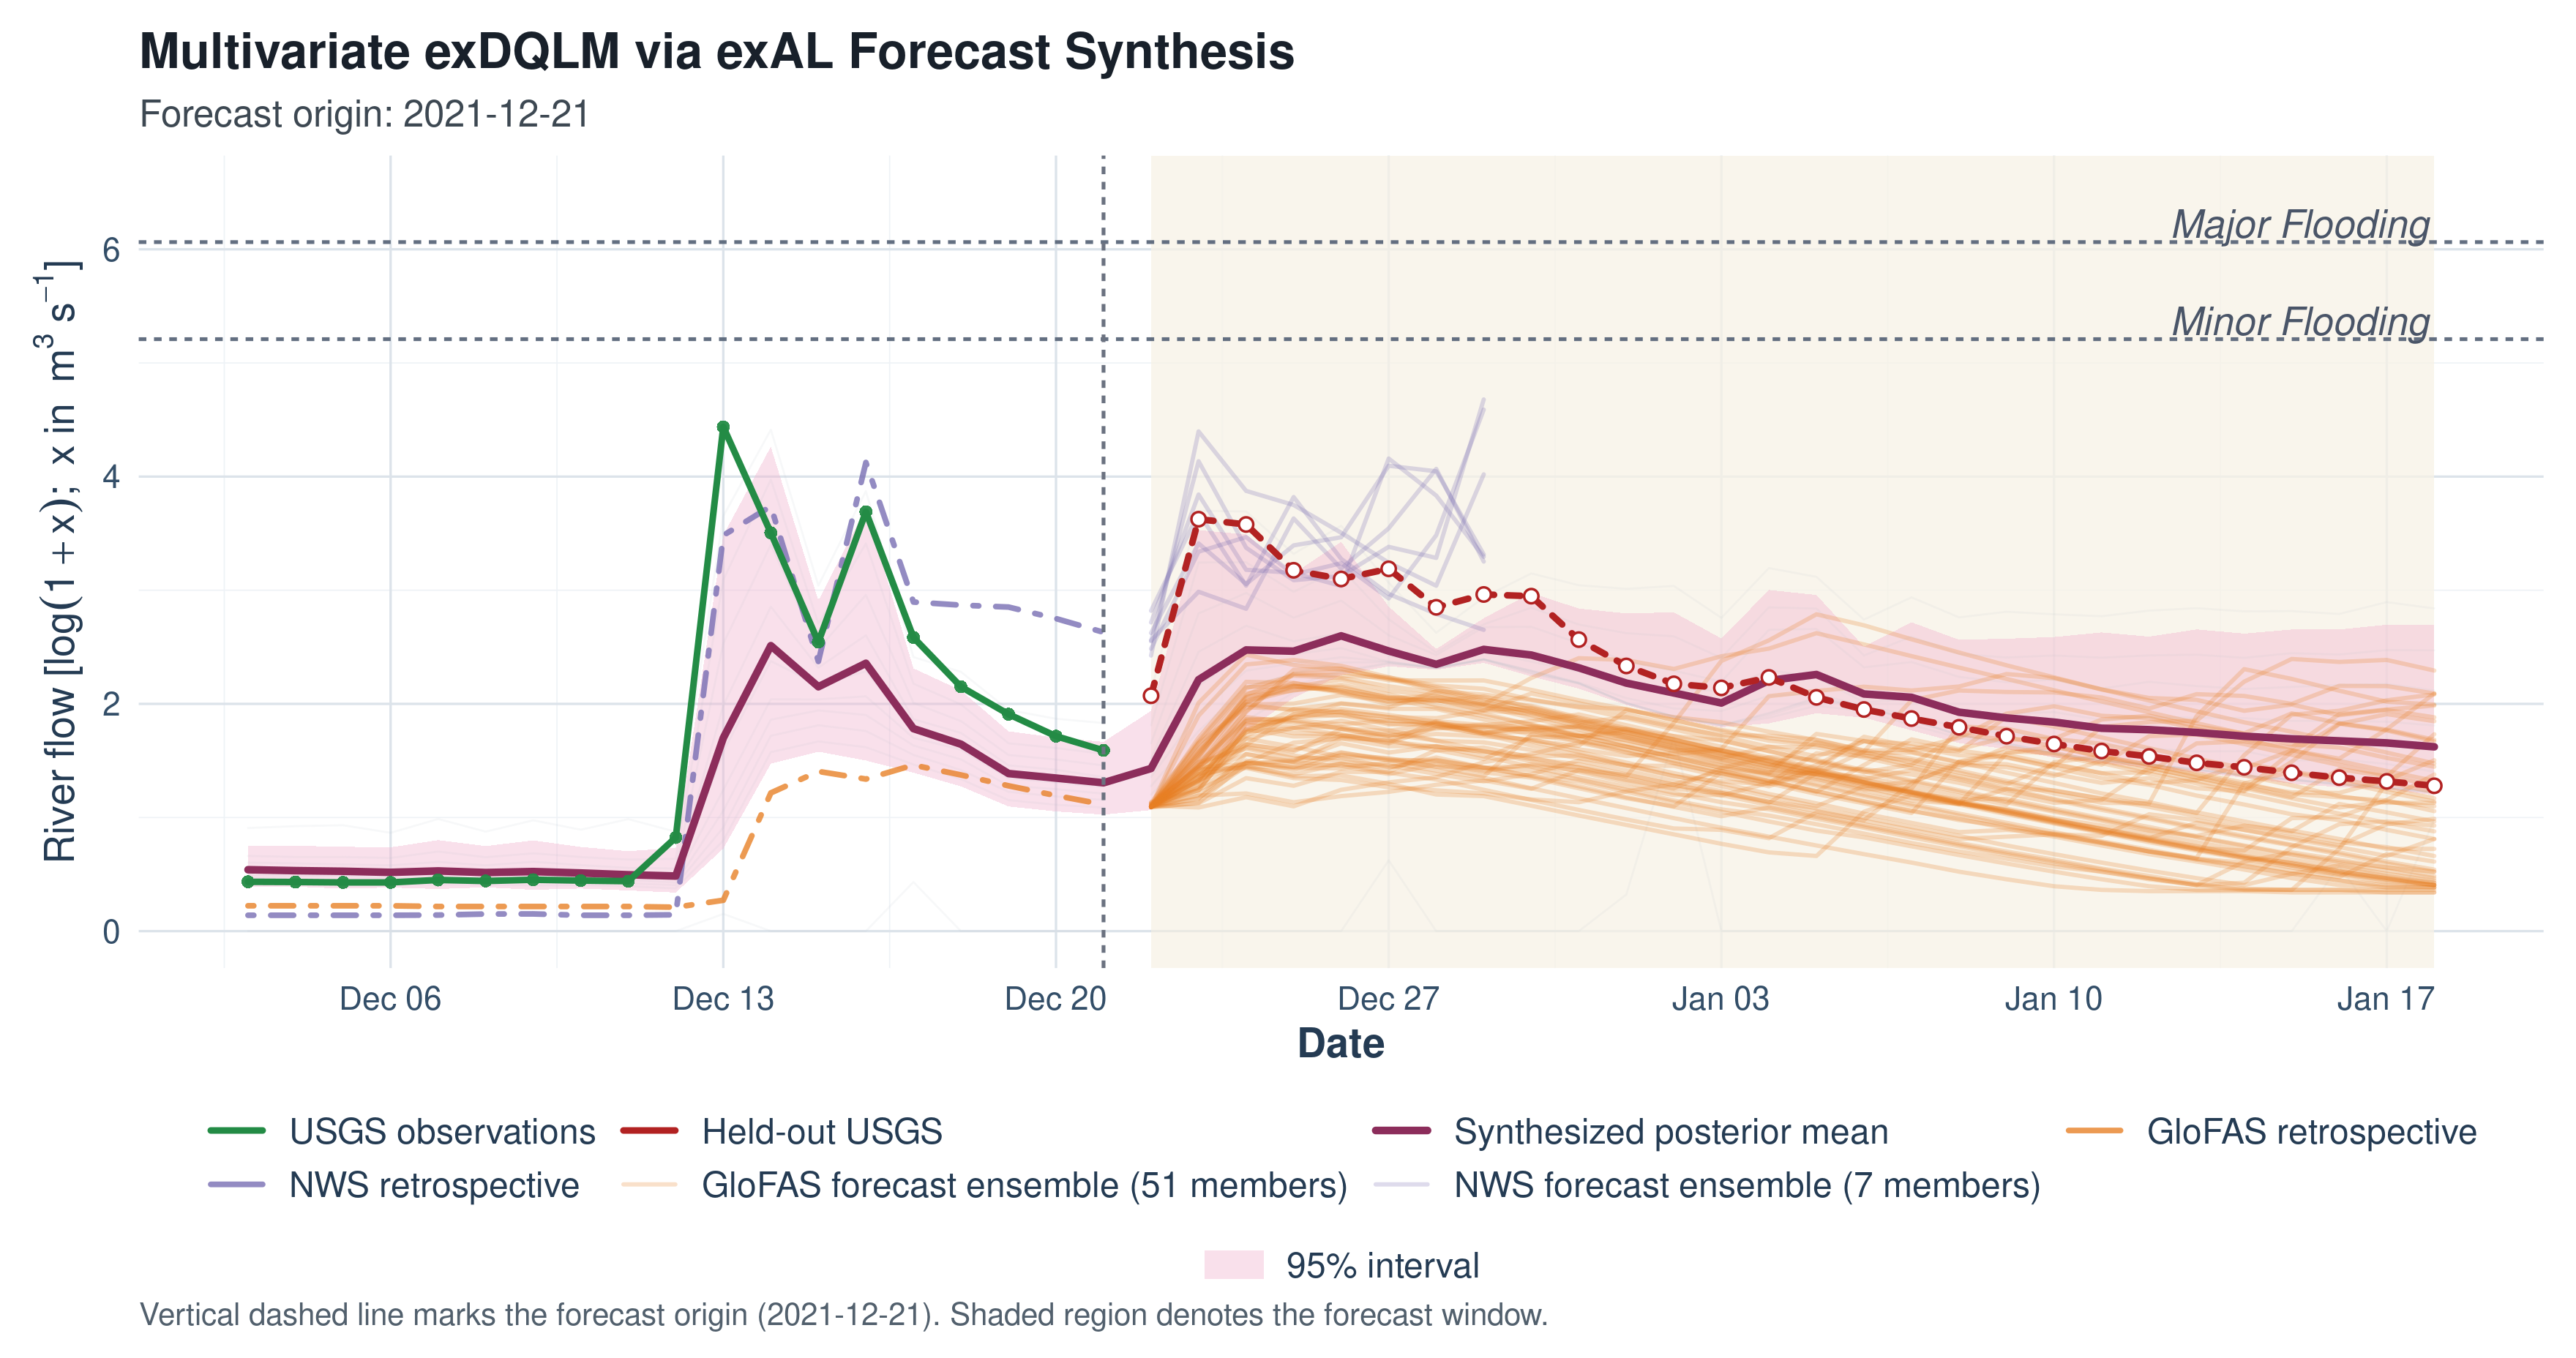
\includegraphics[width=0.76\textwidth]{figures/ch03-environ/cutoff_2021_12_21_multivariate_synthesis_with_reference_ensembles.png}

\medskip
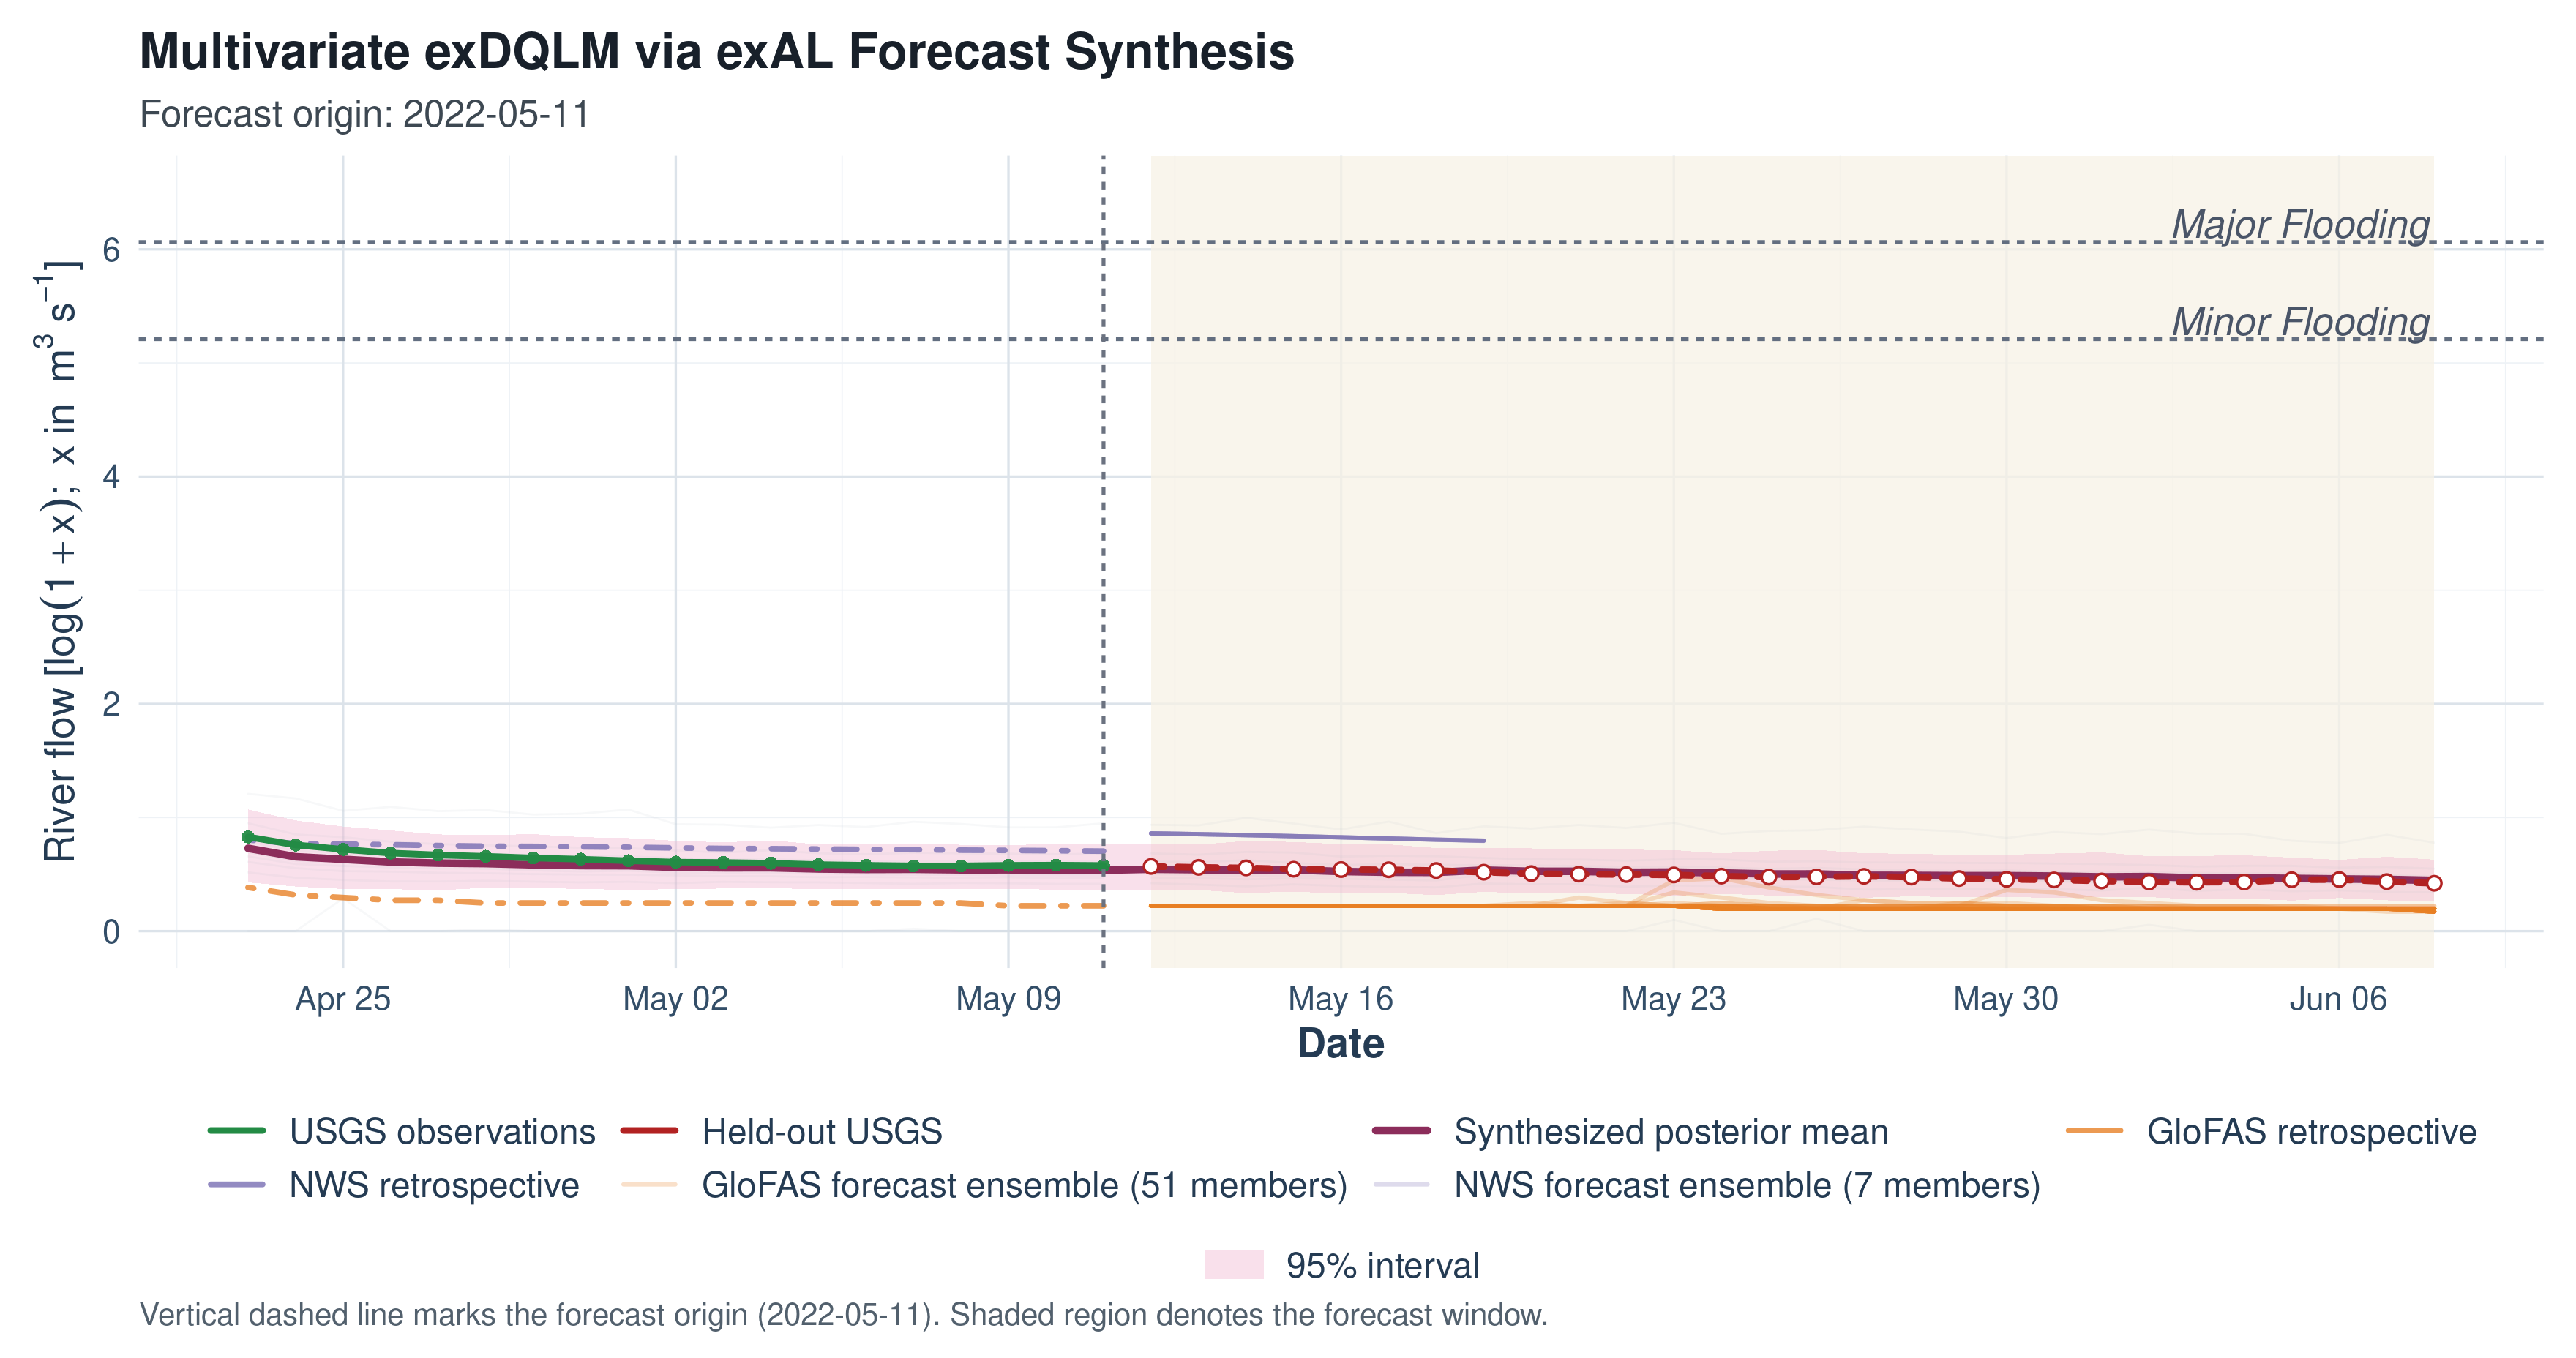
\includegraphics[width=0.76\textwidth]{figures/ch03-environ/cutoff_2022_05_11_multivariate_synthesis_with_reference_ensembles.png}
\caption[Predictive synthesis at the December 2021 and May 2022 cutoffs]{
Predictive synthesis under exAL-M-T1 at the December 21, 2021 (upper) and May
11, 2022 (lower) cutoffs. Colors, bands, quantile curves, and reference overlays
have the same meanings as in Figure~\ref{env:fig:synthsupport_20210123}.
}
\label{env:fig:synthsupport_20211221}
\end{figure}
